\documentclass{standalone}
\usepackage{tikz}
\usetikzlibrary{patterns, positioning}

\begin{document}
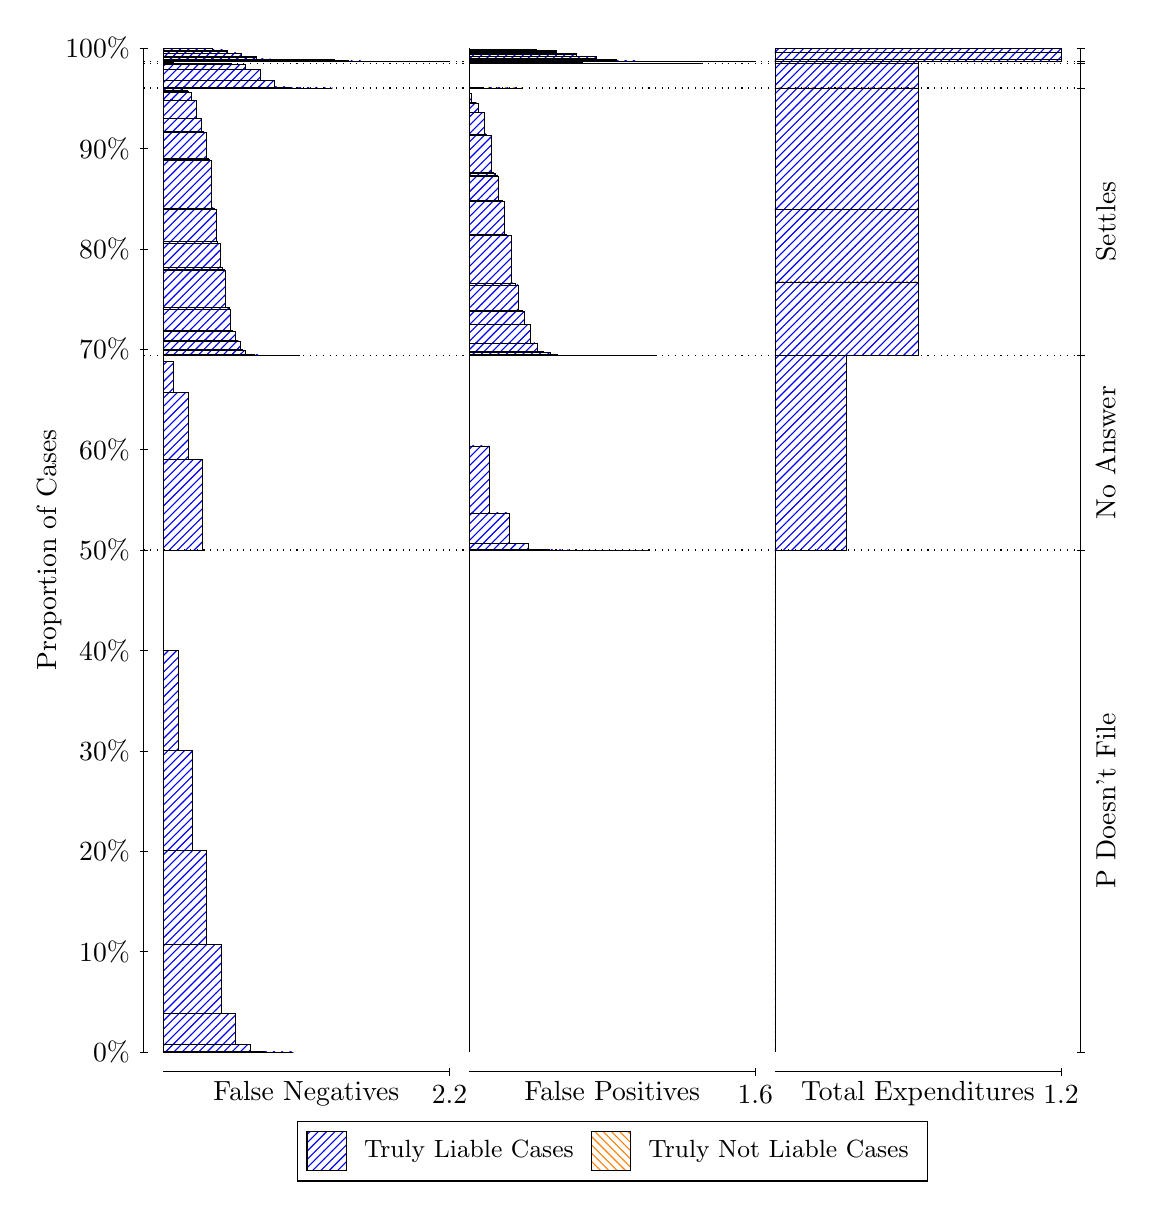
\begin{tikzpicture}
\draw[black, very thin] (1.5,1.75) -- (1.5,14.5);
\node[rotate=90, anchor=center] at (0.3, 8.125) {Proportion of Cases};
\draw[black, very thin] (1.45,1.75) -- (1.55,1.75);
\node[anchor=east] at (1.45, 1.75) {0\%};
\draw[black, very thin] (1.45,3.025) -- (1.55,3.025);
\node[anchor=east] at (1.45, 3.025) {10\%};
\draw[black, very thin] (1.45,4.3) -- (1.55,4.3);
\node[anchor=east] at (1.45, 4.3) {20\%};
\draw[black, very thin] (1.45,5.575) -- (1.55,5.575);
\node[anchor=east] at (1.45, 5.575) {30\%};
\draw[black, very thin] (1.45,6.85) -- (1.55,6.85);
\node[anchor=east] at (1.45, 6.85) {40\%};
\draw[black, very thin] (1.45,8.125) -- (1.55,8.125);
\node[anchor=east] at (1.45, 8.125) {50\%};
\draw[black, very thin] (1.45,9.4) -- (1.55,9.4);
\node[anchor=east] at (1.45, 9.4) {60\%};
\draw[black, very thin] (1.45,10.675) -- (1.55,10.675);
\node[anchor=east] at (1.45, 10.675) {70\%};
\draw[black, very thin] (1.45,11.95) -- (1.55,11.95);
\node[anchor=east] at (1.45, 11.95) {80\%};
\draw[black, very thin] (1.45,13.225) -- (1.55,13.225);
\node[anchor=east] at (1.45, 13.225) {90\%};
\draw[black, very thin] (1.45,14.5) -- (1.55,14.5);
\node[anchor=east] at (1.45, 14.5) {100\%};

\draw[black, very thin] (13.4,1.75) -- (13.4,14.5);
\draw[black, very thin] (13.35,1.75) -- (13.45,1.75);
\node[anchor=west] at (13.35, 1.75) {};
\draw[black, very thin] (13.35,8.125) -- (13.45,8.125);
\node[anchor=west] at (13.35, 8.125) {};
\draw[black, very thin] (13.35,10.6) -- (13.45,10.6);
\node[anchor=west] at (13.35, 10.6) {};
\draw[black, very thin] (13.35,13.993) -- (13.45,13.993);
\node[anchor=west] at (13.35, 13.993) {};
\draw[black, very thin] (13.35,14.3) -- (13.45,14.3);
\node[anchor=west] at (13.35, 14.3) {};
\draw[black, very thin] (13.35,14.331) -- (13.45,14.331);
\node[anchor=west] at (13.35, 14.331) {};
\draw[black, very thin] (13.35,14.5) -- (13.45,14.5);
\node[anchor=west] at (13.35, 14.5) {};

\draw[black, very thin, pattern color=blue, pattern=north east lines] (1.75,1.75) rectangle (3.4015,1.75);
\draw[black, very thin, pattern color=blue, pattern=north east lines] (1.75,1.75) rectangle (3.218,1.7503);
\draw[black, very thin, pattern color=blue, pattern=north east lines] (1.75,1.7503) rectangle (3.0345,1.7583);
\draw[black, very thin, pattern color=blue, pattern=north east lines] (1.75,1.7583) rectangle (2.851,1.8435);
\draw[black, very thin, pattern color=blue, pattern=north east lines] (1.75,1.8435) rectangle (2.6675,2.2369);
\draw[black, very thin, pattern color=blue, pattern=north east lines] (1.75,2.2369) rectangle (2.484,3.1185);
\draw[black, very thin, pattern color=blue, pattern=north east lines] (1.75,3.1185) rectangle (2.3005,4.3083);
\draw[black, very thin, pattern color=blue, pattern=north east lines] (1.75,4.3083) rectangle (2.117,5.5753);
\draw[black, very thin, pattern color=blue, pattern=north east lines] (1.75,5.5753) rectangle (1.9335,6.85);
\draw[black, very thin, pattern color=orange, pattern=north west lines] (1.75,6.85) rectangle (1.75,6.85);
\draw[black, very thin, pattern color=blue, pattern=north east lines] (1.75,6.85) rectangle (1.75,8.125);
\draw[black, very thin, pattern color=blue, pattern=north east lines] (1.75,8.125) rectangle (2.2455,9.2768);
\draw[black, very thin, pattern color=blue, pattern=north east lines] (1.75,9.2768) rectangle (2.062,10.13);
\draw[black, very thin, pattern color=blue, pattern=north east lines] (1.75,10.13) rectangle (1.8785,10.516);
\draw[black, very thin, pattern color=orange, pattern=north west lines] (1.75,10.516) rectangle (1.75,10.516);
\draw[black, very thin, pattern color=blue, pattern=north east lines] (1.75,10.516) rectangle (1.75,10.6);
\draw[black, very thin, pattern color=blue, pattern=north east lines] (1.75,10.6) rectangle (3.4841,10.6);
\draw[black, very thin, pattern color=blue, pattern=north east lines] (1.75,10.6) rectangle (3.4015,10.6);
\draw[black, very thin, pattern color=blue, pattern=north east lines] (1.75,10.6) rectangle (3.3189,10.6);
\draw[black, very thin, pattern color=blue, pattern=north east lines] (1.75,10.6) rectangle (3.3006,10.6);
\draw[black, very thin, pattern color=blue, pattern=north east lines] (1.75,10.6) rectangle (3.2364,10.6);
\draw[black, very thin, pattern color=blue, pattern=north east lines] (1.75,10.6) rectangle (3.218,10.6);
\draw[black, very thin, pattern color=blue, pattern=north east lines] (1.75,10.6) rectangle (3.1538,10.6);
\draw[black, very thin, pattern color=blue, pattern=north east lines] (1.75,10.6) rectangle (3.1354,10.6);
\draw[black, very thin, pattern color=blue, pattern=north east lines] (1.75,10.6) rectangle (3.1171,10.6);
\draw[black, very thin, pattern color=blue, pattern=north east lines] (1.75,10.6) rectangle (3.0712,10.6);
\draw[black, very thin, pattern color=blue, pattern=north east lines] (1.75,10.6) rectangle (3.0529,10.6);
\draw[black, very thin, pattern color=blue, pattern=north east lines] (1.75,10.6) rectangle (3.0345,10.6);
\draw[black, very thin, pattern color=blue, pattern=north east lines] (1.75,10.6) rectangle (2.9886,10.6);
\draw[black, very thin, pattern color=blue, pattern=north east lines] (1.75,10.6) rectangle (2.9703,10.603);
\draw[black, very thin, pattern color=blue, pattern=north east lines] (1.75,10.603) rectangle (2.9519,10.603);
\draw[black, very thin, pattern color=blue, pattern=north east lines] (1.75,10.603) rectangle (2.9336,10.603);
\draw[black, very thin, pattern color=blue, pattern=north east lines] (1.75,10.603) rectangle (2.9061,10.612);
\draw[black, very thin, pattern color=blue, pattern=north east lines] (1.75,10.612) rectangle (2.8877,10.612);
\draw[black, very thin, pattern color=blue, pattern=north east lines] (1.75,10.612) rectangle (2.8694,10.613);
\draw[black, very thin, pattern color=blue, pattern=north east lines] (1.75,10.613) rectangle (2.851,10.613);
\draw[black, very thin, pattern color=blue, pattern=north east lines] (1.75,10.613) rectangle (2.8051,10.614);
\draw[black, very thin, pattern color=blue, pattern=north east lines] (1.75,10.614) rectangle (2.7868,10.662);
\draw[black, very thin, pattern color=blue, pattern=north east lines] (1.75,10.662) rectangle (2.7684,10.667);
\draw[black, very thin, pattern color=blue, pattern=north east lines] (1.75,10.667) rectangle (2.7501,10.669);
\draw[black, very thin, pattern color=blue, pattern=north east lines] (1.75,10.669) rectangle (2.7226,10.778);
\draw[black, very thin, pattern color=blue, pattern=north east lines] (1.75,10.778) rectangle (2.7042,10.781);
\draw[black, very thin, pattern color=blue, pattern=north east lines] (1.75,10.781) rectangle (2.6859,10.791);
\draw[black, very thin, pattern color=blue, pattern=north east lines] (1.75,10.791) rectangle (2.6675,10.793);
\draw[black, very thin, pattern color=blue, pattern=north east lines] (1.75,10.793) rectangle (2.6583,10.907);
\draw[black, very thin, pattern color=blue, pattern=north east lines] (1.75,10.907) rectangle (2.6216,10.913);
\draw[black, very thin, pattern color=blue, pattern=north east lines] (1.75,10.913) rectangle (2.6033,11.185);
\draw[black, very thin, pattern color=blue, pattern=north east lines] (1.75,11.185) rectangle (2.5849,11.204);
\draw[black, very thin, pattern color=blue, pattern=north east lines] (1.75,11.204) rectangle (2.5666,11.208);
\draw[black, very thin, pattern color=blue, pattern=north east lines] (1.75,11.208) rectangle (2.5391,11.673);
\draw[black, very thin, pattern color=blue, pattern=north east lines] (1.75,11.673) rectangle (2.5207,11.685);
\draw[black, very thin, pattern color=blue, pattern=north east lines] (1.75,11.685) rectangle (2.5024,11.716);
\draw[black, very thin, pattern color=blue, pattern=north east lines] (1.75,11.716) rectangle (2.484,11.718);
\draw[black, very thin, pattern color=blue, pattern=north east lines] (1.75,11.718) rectangle (2.4748,12.021);
\draw[black, very thin, pattern color=blue, pattern=north east lines] (1.75,12.021) rectangle (2.4381,12.044);
\draw[black, very thin, pattern color=blue, pattern=north east lines] (1.75,12.044) rectangle (2.4198,12.455);
\draw[black, very thin, pattern color=blue, pattern=north east lines] (1.75,12.455) rectangle (2.4014,12.468);
\draw[black, very thin, pattern color=blue, pattern=north east lines] (1.75,12.468) rectangle (2.3831,12.469);
\draw[black, very thin, pattern color=blue, pattern=north east lines] (1.75,12.469) rectangle (2.3556,13.076);
\draw[black, very thin, pattern color=blue, pattern=north east lines] (1.75,13.076) rectangle (2.3372,13.085);
\draw[black, very thin, pattern color=blue, pattern=north east lines] (1.75,13.085) rectangle (2.3189,13.103);
\draw[black, very thin, pattern color=blue, pattern=north east lines] (1.75,13.103) rectangle (2.3005,13.103);
\draw[black, very thin, pattern color=blue, pattern=north east lines] (1.75,13.103) rectangle (2.2913,13.425);
\draw[black, very thin, pattern color=blue, pattern=north east lines] (1.75,13.425) rectangle (2.2546,13.443);
\draw[black, very thin, pattern color=blue, pattern=north east lines] (1.75,13.443) rectangle (2.2363,13.605);
\draw[black, very thin, pattern color=blue, pattern=north east lines] (1.75,13.605) rectangle (2.2179,13.607);
\draw[black, very thin, pattern color=blue, pattern=north east lines] (1.75,13.607) rectangle (2.1996,13.607);
\draw[black, very thin, pattern color=blue, pattern=north east lines] (1.75,13.607) rectangle (2.1721,13.839);
\draw[black, very thin, pattern color=blue, pattern=north east lines] (1.75,13.839) rectangle (2.1537,13.84);
\draw[black, very thin, pattern color=blue, pattern=north east lines] (1.75,13.84) rectangle (2.1354,13.842);
\draw[black, very thin, pattern color=blue, pattern=north east lines] (1.75,13.842) rectangle (2.117,13.842);
\draw[black, very thin, pattern color=blue, pattern=north east lines] (1.75,13.842) rectangle (2.1078,13.944);
\draw[black, very thin, pattern color=blue, pattern=north east lines] (1.75,13.944) rectangle (2.0711,13.946);
\draw[black, very thin, pattern color=blue, pattern=north east lines] (1.75,13.946) rectangle (2.0528,13.961);
\draw[black, very thin, pattern color=blue, pattern=north east lines] (1.75,13.961) rectangle (2.0344,13.961);
\draw[black, very thin, pattern color=blue, pattern=north east lines] (1.75,13.961) rectangle (2.0161,13.961);
\draw[black, very thin, pattern color=blue, pattern=north east lines] (1.75,13.961) rectangle (1.9886,13.984);
\draw[black, very thin, pattern color=blue, pattern=north east lines] (1.75,13.984) rectangle (1.9702,13.984);
\draw[black, very thin, pattern color=blue, pattern=north east lines] (1.75,13.984) rectangle (1.9519,13.984);
\draw[black, very thin, pattern color=blue, pattern=north east lines] (1.75,13.984) rectangle (1.9335,13.984);
\draw[black, very thin, pattern color=blue, pattern=north east lines] (1.75,13.984) rectangle (1.9243,13.992);
\draw[black, very thin, pattern color=blue, pattern=north east lines] (1.75,13.992) rectangle (1.8876,13.992);
\draw[black, very thin, pattern color=blue, pattern=north east lines] (1.75,13.992) rectangle (1.8693,13.993);
\draw[black, very thin, pattern color=blue, pattern=north east lines] (1.75,13.993) rectangle (1.8509,13.993);
\draw[black, very thin, pattern color=blue, pattern=north east lines] (1.75,13.993) rectangle (1.8326,13.993);
\draw[black, very thin, pattern color=blue, pattern=north east lines] (1.75,13.993) rectangle (1.8051,13.993);
\draw[black, very thin, pattern color=blue, pattern=north east lines] (1.75,13.993) rectangle (1.7867,13.993);
\draw[black, very thin, pattern color=blue, pattern=north east lines] (1.75,13.993) rectangle (1.7684,13.993);
\draw[black, very thin, pattern color=orange, pattern=north west lines] (1.75,13.993) rectangle (1.75,13.993);
\draw[black, very thin, pattern color=blue, pattern=north east lines] (1.75,13.993) rectangle (1.75,13.993);
\draw[black, very thin, pattern color=blue, pattern=north east lines] (1.75,13.993) rectangle (3.897,13.993);
\draw[black, very thin, pattern color=blue, pattern=north east lines] (1.75,13.993) rectangle (3.7135,13.993);
\draw[black, very thin, pattern color=blue, pattern=north east lines] (1.75,13.993) rectangle (3.53,13.994);
\draw[black, very thin, pattern color=blue, pattern=north east lines] (1.75,13.994) rectangle (3.3465,14.006);
\draw[black, very thin, pattern color=blue, pattern=north east lines] (1.75,14.006) rectangle (3.163,14.091);
\draw[black, very thin, pattern color=blue, pattern=north east lines] (1.75,14.091) rectangle (2.9795,14.232);
\draw[black, very thin, pattern color=blue, pattern=north east lines] (1.75,14.232) rectangle (2.796,14.293);
\draw[black, very thin, pattern color=blue, pattern=north east lines] (1.75,14.293) rectangle (2.6125,14.3);
\draw[black, very thin, pattern color=blue, pattern=north east lines] (1.75,14.3) rectangle (2.429,14.3);
\draw[black, very thin, pattern color=blue, pattern=north east lines] (1.75,14.3) rectangle (2.2455,14.3);
\draw[black, very thin, pattern color=orange, pattern=north west lines] (1.75,14.3) rectangle (1.75,14.3);
\draw[black, very thin, pattern color=blue, pattern=north east lines] (1.75,14.3) rectangle (2.2455,14.3);
\draw[black, very thin, pattern color=blue, pattern=north east lines] (1.75,14.3) rectangle (2.062,14.302);
\draw[black, very thin, pattern color=blue, pattern=north east lines] (1.75,14.302) rectangle (1.8785,14.313);
\draw[black, very thin, pattern color=orange, pattern=north west lines] (1.75,14.313) rectangle (1.75,14.313);
\draw[black, very thin, pattern color=blue, pattern=north east lines] (1.75,14.313) rectangle (1.75,14.331);
\draw[black, very thin, pattern color=blue, pattern=north east lines] (1.75,14.331) rectangle (5.3833,14.331);
\draw[black, very thin, pattern color=blue, pattern=north east lines] (1.75,14.331) rectangle (5.1998,14.331);
\draw[black, very thin, pattern color=blue, pattern=north east lines] (1.75,14.331) rectangle (5.0163,14.331);
\draw[black, very thin, pattern color=blue, pattern=north east lines] (1.75,14.331) rectangle (5.0163,14.331);
\draw[black, very thin, pattern color=blue, pattern=north east lines] (1.75,14.331) rectangle (4.8328,14.331);
\draw[black, very thin, pattern color=blue, pattern=north east lines] (1.75,14.331) rectangle (4.6493,14.331);
\draw[black, very thin, pattern color=blue, pattern=north east lines] (1.75,14.331) rectangle (4.4658,14.332);
\draw[black, very thin, pattern color=blue, pattern=north east lines] (1.75,14.332) rectangle (4.2823,14.338);
\draw[black, very thin, pattern color=blue, pattern=north east lines] (1.75,14.338) rectangle (4.0988,14.341);
\draw[black, very thin, pattern color=blue, pattern=north east lines] (1.75,14.341) rectangle (4.0988,14.347);
\draw[black, very thin, pattern color=blue, pattern=north east lines] (1.75,14.347) rectangle (4.0254,14.347);
\draw[black, very thin, pattern color=blue, pattern=north east lines] (1.75,14.347) rectangle (3.9153,14.351);
\draw[black, very thin, pattern color=blue, pattern=north east lines] (1.75,14.351) rectangle (3.9153,14.351);
\draw[black, very thin, pattern color=blue, pattern=north east lines] (1.75,14.351) rectangle (3.8419,14.351);
\draw[black, very thin, pattern color=blue, pattern=north east lines] (1.75,14.351) rectangle (3.7318,14.351);
\draw[black, very thin, pattern color=blue, pattern=north east lines] (1.75,14.351) rectangle (3.6584,14.351);
\draw[black, very thin, pattern color=blue, pattern=north east lines] (1.75,14.351) rectangle (3.5483,14.351);
\draw[black, very thin, pattern color=blue, pattern=north east lines] (1.75,14.351) rectangle (3.5483,14.351);
\draw[black, very thin, pattern color=blue, pattern=north east lines] (1.75,14.351) rectangle (3.4749,14.351);
\draw[black, very thin, pattern color=blue, pattern=north east lines] (1.75,14.351) rectangle (3.4749,14.351);
\draw[black, very thin, pattern color=blue, pattern=north east lines] (1.75,14.351) rectangle (3.3648,14.351);
\draw[black, very thin, pattern color=blue, pattern=north east lines] (1.75,14.351) rectangle (3.3648,14.351);
\draw[black, very thin, pattern color=blue, pattern=north east lines] (1.75,14.351) rectangle (3.2914,14.352);
\draw[black, very thin, pattern color=blue, pattern=north east lines] (1.75,14.352) rectangle (3.2914,14.352);
\draw[black, very thin, pattern color=blue, pattern=north east lines] (1.75,14.352) rectangle (3.1813,14.352);
\draw[black, very thin, pattern color=blue, pattern=north east lines] (1.75,14.352) rectangle (3.1079,14.362);
\draw[black, very thin, pattern color=blue, pattern=north east lines] (1.75,14.362) rectangle (2.9978,14.362);
\draw[black, very thin, pattern color=blue, pattern=north east lines] (1.75,14.362) rectangle (2.9244,14.377);
\draw[black, very thin, pattern color=blue, pattern=north east lines] (1.75,14.377) rectangle (2.9244,14.395);
\draw[black, very thin, pattern color=blue, pattern=north east lines] (1.75,14.395) rectangle (2.7409,14.439);
\draw[black, very thin, pattern color=blue, pattern=north east lines] (1.75,14.439) rectangle (2.5574,14.457);
\draw[black, very thin, pattern color=blue, pattern=north east lines] (1.75,14.457) rectangle (2.5574,14.457);
\draw[black, very thin, pattern color=blue, pattern=north east lines] (1.75,14.457) rectangle (2.5574,14.475);
\draw[black, very thin, pattern color=blue, pattern=north east lines] (1.75,14.475) rectangle (2.3739,14.493);
\draw[black, very thin, pattern color=blue, pattern=north east lines] (1.75,14.493) rectangle (2.3739,14.494);
\draw[black, very thin, pattern color=blue, pattern=north east lines] (1.75,14.494) rectangle (2.1904,14.496);
\draw[black, very thin, pattern color=blue, pattern=north east lines] (1.75,14.496) rectangle (2.1904,14.496);
\draw[black, very thin, pattern color=blue, pattern=north east lines] (1.75,14.496) rectangle (2.1904,14.499);
\draw[black, very thin, pattern color=blue, pattern=north east lines] (1.75,14.499) rectangle (2.0069,14.5);
\draw[black, very thin, pattern color=blue, pattern=north east lines] (1.75,14.5) rectangle (2.0069,14.5);
\draw[black, very thin, pattern color=blue, pattern=north east lines] (1.75,14.5) rectangle (1.8234,14.5);
\draw[black, very thin, pattern color=blue, pattern=north east lines] (1.75,14.5) rectangle (1.8234,14.5);
\draw[black, very thin, pattern color=orange, pattern=north west lines] (1.75,14.5) rectangle (1.75,14.5);
\draw[black, very thin, pattern color=blue, pattern=north east lines] (1.75,14.5) rectangle (1.75,14.5);
\draw[black, very thin, pattern color=orange, pattern=north west lines] (5.6333,1.75) rectangle (5.6333,1.75);
\draw[black, very thin, pattern color=blue, pattern=north east lines] (5.6333,1.75) rectangle (5.6333,8.125);
\draw[black, very thin, pattern color=orange, pattern=north west lines] (5.6333,8.125) rectangle (7.9042,8.125);
\draw[black, very thin, pattern color=blue, pattern=north east lines] (5.6333,8.125) rectangle (7.9042,8.125);
\draw[black, very thin, pattern color=blue, pattern=north east lines] (5.6333,8.125) rectangle (7.6519,8.125);
\draw[black, very thin, pattern color=blue, pattern=north east lines] (5.6333,8.125) rectangle (7.3995,8.125);
\draw[black, very thin, pattern color=blue, pattern=north east lines] (5.6333,8.125) rectangle (7.1472,8.125);
\draw[black, very thin, pattern color=blue, pattern=north east lines] (5.6333,8.125) rectangle (6.8949,8.1251);
\draw[black, very thin, pattern color=blue, pattern=north east lines] (5.6333,8.1251) rectangle (6.6426,8.1306);
\draw[black, very thin, pattern color=blue, pattern=north east lines] (5.6333,8.1306) rectangle (6.3903,8.2098);
\draw[black, very thin, pattern color=blue, pattern=north east lines] (5.6333,8.2098) rectangle (6.138,8.5952);
\draw[black, very thin, pattern color=blue, pattern=north east lines] (5.6333,8.5952) rectangle (5.8856,9.4485);
\draw[black, very thin, pattern color=blue, pattern=north east lines] (5.6333,9.4485) rectangle (5.6333,10.6);
\draw[black, very thin, pattern color=orange, pattern=north west lines] (5.6333,10.6) rectangle (8.0177,10.6);
\draw[black, very thin, pattern color=blue, pattern=north east lines] (5.6333,10.6) rectangle (8.0177,10.6);
\draw[black, very thin, pattern color=blue, pattern=north east lines] (5.6333,10.6) rectangle (7.7654,10.6);
\draw[black, very thin, pattern color=orange, pattern=north west lines] (5.6333,10.6) rectangle (7.6771,10.6);
\draw[black, very thin, pattern color=blue, pattern=north east lines] (5.6333,10.6) rectangle (7.6771,10.6);
\draw[black, very thin, pattern color=orange, pattern=north west lines] (5.6333,10.6) rectangle (7.5635,10.6);
\draw[black, very thin, pattern color=blue, pattern=north east lines] (5.6333,10.6) rectangle (7.5635,10.6);
\draw[black, very thin, pattern color=blue, pattern=north east lines] (5.6333,10.6) rectangle (7.5131,10.6);
\draw[black, very thin, pattern color=orange, pattern=north west lines] (5.6333,10.6) rectangle (7.45,10.6);
\draw[black, very thin, pattern color=blue, pattern=north east lines] (5.6333,10.6) rectangle (7.45,10.6);
\draw[black, very thin, pattern color=blue, pattern=north east lines] (5.6333,10.6) rectangle (7.4248,10.6);
\draw[black, very thin, pattern color=orange, pattern=north west lines] (5.6333,10.6) rectangle (7.3365,10.6);
\draw[black, very thin, pattern color=blue, pattern=north east lines] (5.6333,10.6) rectangle (7.3365,10.6);
\draw[black, very thin, pattern color=blue, pattern=north east lines] (5.6333,10.6) rectangle (7.3112,10.6);
\draw[black, very thin, pattern color=blue, pattern=north east lines] (5.6333,10.6) rectangle (7.2608,10.6);
\draw[black, very thin, pattern color=orange, pattern=north west lines] (5.6333,10.6) rectangle (7.2229,10.6);
\draw[black, very thin, pattern color=blue, pattern=north east lines] (5.6333,10.6) rectangle (7.2229,10.6);
\draw[black, very thin, pattern color=blue, pattern=north east lines] (5.6333,10.6) rectangle (7.1977,10.6);
\draw[black, very thin, pattern color=blue, pattern=north east lines] (5.6333,10.6) rectangle (7.1725,10.6);
\draw[black, very thin, pattern color=orange, pattern=north west lines] (5.6333,10.6) rectangle (7.1094,10.6);
\draw[black, very thin, pattern color=blue, pattern=north east lines] (5.6333,10.6) rectangle (7.1094,10.6);
\draw[black, very thin, pattern color=blue, pattern=north east lines] (5.6333,10.6) rectangle (7.0841,10.6);
\draw[black, very thin, pattern color=blue, pattern=north east lines] (5.6333,10.6) rectangle (7.0589,10.6);
\draw[black, very thin, pattern color=blue, pattern=north east lines] (5.6333,10.6) rectangle (7.0084,10.6);
\draw[black, very thin, pattern color=orange, pattern=north west lines] (5.6333,10.6) rectangle (6.9958,10.6);
\draw[black, very thin, pattern color=blue, pattern=north east lines] (5.6333,10.6) rectangle (6.9958,10.6);
\draw[black, very thin, pattern color=blue, pattern=north east lines] (5.6333,10.6) rectangle (6.9706,10.6);
\draw[black, very thin, pattern color=blue, pattern=north east lines] (5.6333,10.6) rectangle (6.9454,10.6);
\draw[black, very thin, pattern color=blue, pattern=north east lines] (5.6333,10.6) rectangle (6.9201,10.601);
\draw[black, very thin, pattern color=orange, pattern=north west lines] (5.6333,10.601) rectangle (6.8823,10.601);
\draw[black, very thin, pattern color=blue, pattern=north east lines] (5.6333,10.601) rectangle (6.8823,10.601);
\draw[black, very thin, pattern color=blue, pattern=north east lines] (5.6333,10.601) rectangle (6.8571,10.601);
\draw[black, very thin, pattern color=blue, pattern=north east lines] (5.6333,10.601) rectangle (6.8318,10.601);
\draw[black, very thin, pattern color=blue, pattern=north east lines] (5.6333,10.601) rectangle (6.8066,10.601);
\draw[black, very thin, pattern color=blue, pattern=north east lines] (5.6333,10.601) rectangle (6.7561,10.61);
\draw[black, very thin, pattern color=blue, pattern=north east lines] (5.6333,10.61) rectangle (6.7435,10.61);
\draw[black, very thin, pattern color=blue, pattern=north east lines] (5.6333,10.61) rectangle (6.7183,10.61);
\draw[black, very thin, pattern color=blue, pattern=north east lines] (5.6333,10.61) rectangle (6.6931,10.61);
\draw[black, very thin, pattern color=blue, pattern=north east lines] (5.6333,10.61) rectangle (6.6678,10.632);
\draw[black, very thin, pattern color=blue, pattern=north east lines] (5.6333,10.632) rectangle (6.63,10.632);
\draw[black, very thin, pattern color=blue, pattern=north east lines] (5.6333,10.632) rectangle (6.6047,10.632);
\draw[black, very thin, pattern color=blue, pattern=north east lines] (5.6333,10.632) rectangle (6.5795,10.647);
\draw[black, very thin, pattern color=blue, pattern=north east lines] (5.6333,10.647) rectangle (6.5543,10.65);
\draw[black, very thin, pattern color=blue, pattern=north east lines] (5.6333,10.65) rectangle (6.5038,10.752);
\draw[black, very thin, pattern color=blue, pattern=north east lines] (5.6333,10.752) rectangle (6.4912,10.752);
\draw[black, very thin, pattern color=blue, pattern=north east lines] (5.6333,10.752) rectangle (6.466,10.754);
\draw[black, very thin, pattern color=blue, pattern=north east lines] (5.6333,10.754) rectangle (6.4407,10.755);
\draw[black, very thin, pattern color=blue, pattern=north east lines] (5.6333,10.755) rectangle (6.4155,10.987);
\draw[black, very thin, pattern color=blue, pattern=north east lines] (5.6333,10.987) rectangle (6.3777,10.987);
\draw[black, very thin, pattern color=blue, pattern=north east lines] (5.6333,10.987) rectangle (6.3524,10.988);
\draw[black, very thin, pattern color=blue, pattern=north east lines] (5.6333,10.988) rectangle (6.3272,11.151);
\draw[black, very thin, pattern color=blue, pattern=north east lines] (5.6333,11.151) rectangle (6.302,11.168);
\draw[black, very thin, pattern color=blue, pattern=north east lines] (5.6333,11.168) rectangle (6.2515,11.491);
\draw[black, very thin, pattern color=blue, pattern=north east lines] (5.6333,11.491) rectangle (6.2389,11.491);
\draw[black, very thin, pattern color=blue, pattern=north east lines] (5.6333,11.491) rectangle (6.2137,11.509);
\draw[black, very thin, pattern color=blue, pattern=north east lines] (5.6333,11.509) rectangle (6.1884,11.518);
\draw[black, very thin, pattern color=blue, pattern=north east lines] (5.6333,11.518) rectangle (6.1632,12.124);
\draw[black, very thin, pattern color=blue, pattern=north east lines] (5.6333,12.124) rectangle (6.1253,12.126);
\draw[black, very thin, pattern color=blue, pattern=north east lines] (5.6333,12.126) rectangle (6.1001,12.138);
\draw[black, very thin, pattern color=blue, pattern=north east lines] (5.6333,12.138) rectangle (6.0749,12.549);
\draw[black, very thin, pattern color=blue, pattern=north east lines] (5.6333,12.549) rectangle (6.0497,12.572);
\draw[black, very thin, pattern color=blue, pattern=north east lines] (5.6333,12.572) rectangle (5.9992,12.876);
\draw[black, very thin, pattern color=blue, pattern=north east lines] (5.6333,12.876) rectangle (5.9866,12.878);
\draw[black, very thin, pattern color=blue, pattern=north east lines] (5.6333,12.878) rectangle (5.9613,12.909);
\draw[black, very thin, pattern color=blue, pattern=north east lines] (5.6333,12.909) rectangle (5.9361,12.92);
\draw[black, very thin, pattern color=blue, pattern=north east lines] (5.6333,12.92) rectangle (5.9109,13.386);
\draw[black, very thin, pattern color=blue, pattern=north east lines] (5.6333,13.386) rectangle (5.873,13.389);
\draw[black, very thin, pattern color=blue, pattern=north east lines] (5.6333,13.389) rectangle (5.8478,13.409);
\draw[black, very thin, pattern color=blue, pattern=north east lines] (5.6333,13.409) rectangle (5.8226,13.681);
\draw[black, very thin, pattern color=blue, pattern=north east lines] (5.6333,13.681) rectangle (5.7973,13.687);
\draw[black, very thin, pattern color=blue, pattern=north east lines] (5.6333,13.687) rectangle (5.7469,13.8);
\draw[black, very thin, pattern color=blue, pattern=north east lines] (5.6333,13.8) rectangle (5.7343,13.802);
\draw[black, very thin, pattern color=blue, pattern=north east lines] (5.6333,13.802) rectangle (5.709,13.812);
\draw[black, very thin, pattern color=blue, pattern=north east lines] (5.6333,13.812) rectangle (5.6838,13.815);
\draw[black, very thin, pattern color=blue, pattern=north east lines] (5.6333,13.815) rectangle (5.6586,13.924);
\draw[black, very thin, pattern color=blue, pattern=north east lines] (5.6333,13.924) rectangle (5.6333,13.993);
\draw[black, very thin, pattern color=orange, pattern=north west lines] (5.6333,13.993) rectangle (6.3146,13.993);
\draw[black, very thin, pattern color=blue, pattern=north east lines] (5.6333,13.993) rectangle (6.3146,13.993);
\draw[black, very thin, pattern color=blue, pattern=north east lines] (5.6333,13.993) rectangle (6.0623,13.993);
\draw[black, very thin, pattern color=blue, pattern=north east lines] (5.6333,13.993) rectangle (5.81,14.001);
\draw[black, very thin, pattern color=blue, pattern=north east lines] (5.6333,14.001) rectangle (5.6333,14.3);
\draw[black, very thin, pattern color=orange, pattern=north west lines] (5.6333,14.3) rectangle (8.5854,14.3);
\draw[black, very thin, pattern color=blue, pattern=north east lines] (5.6333,14.3) rectangle (8.5854,14.3);
\draw[black, very thin, pattern color=blue, pattern=north east lines] (5.6333,14.3) rectangle (8.3331,14.3);
\draw[black, very thin, pattern color=blue, pattern=north east lines] (5.6333,14.3) rectangle (8.0808,14.3);
\draw[black, very thin, pattern color=blue, pattern=north east lines] (5.6333,14.3) rectangle (7.8285,14.3);
\draw[black, very thin, pattern color=blue, pattern=north east lines] (5.6333,14.3) rectangle (7.5762,14.3);
\draw[black, very thin, pattern color=blue, pattern=north east lines] (5.6333,14.3) rectangle (7.3238,14.304);
\draw[black, very thin, pattern color=blue, pattern=north east lines] (5.6333,14.304) rectangle (7.0715,14.318);
\draw[black, very thin, pattern color=blue, pattern=north east lines] (5.6333,14.318) rectangle (6.8192,14.328);
\draw[black, very thin, pattern color=blue, pattern=north east lines] (5.6333,14.328) rectangle (6.5669,14.331);
\draw[black, very thin, pattern color=blue, pattern=north east lines] (5.6333,14.331) rectangle (6.3146,14.331);
\draw[black, very thin, pattern color=orange, pattern=north west lines] (5.6333,14.331) rectangle (9.2667,14.331);
\draw[black, very thin, pattern color=blue, pattern=north east lines] (5.6333,14.331) rectangle (9.2667,14.331);
\draw[black, very thin, pattern color=orange, pattern=north west lines] (5.6333,14.331) rectangle (9.0144,14.331);
\draw[black, very thin, pattern color=blue, pattern=north east lines] (5.6333,14.331) rectangle (9.0144,14.331);
\draw[black, very thin, pattern color=orange, pattern=north west lines] (5.6333,14.331) rectangle (8.762,14.331);
\draw[black, very thin, pattern color=blue, pattern=north east lines] (5.6333,14.331) rectangle (8.762,14.331);
\draw[black, very thin, pattern color=blue, pattern=north east lines] (5.6333,14.331) rectangle (8.5097,14.331);
\draw[black, very thin, pattern color=orange, pattern=north west lines] (5.6333,14.331) rectangle (8.5097,14.331);
\draw[black, very thin, pattern color=blue, pattern=north east lines] (5.6333,14.331) rectangle (8.5097,14.331);
\draw[black, very thin, pattern color=blue, pattern=north east lines] (5.6333,14.331) rectangle (8.2574,14.331);
\draw[black, very thin, pattern color=orange, pattern=north west lines] (5.6333,14.331) rectangle (8.2574,14.331);
\draw[black, very thin, pattern color=blue, pattern=north east lines] (5.6333,14.331) rectangle (8.2574,14.331);
\draw[black, very thin, pattern color=blue, pattern=north east lines] (5.6333,14.331) rectangle (8.0051,14.331);
\draw[black, very thin, pattern color=orange, pattern=north west lines] (5.6333,14.331) rectangle (8.0051,14.331);
\draw[black, very thin, pattern color=blue, pattern=north east lines] (5.6333,14.331) rectangle (8.0051,14.331);
\draw[black, very thin, pattern color=blue, pattern=north east lines] (5.6333,14.331) rectangle (7.7528,14.333);
\draw[black, very thin, pattern color=orange, pattern=north west lines] (5.6333,14.333) rectangle (7.7528,14.333);
\draw[black, very thin, pattern color=blue, pattern=north east lines] (5.6333,14.333) rectangle (7.7528,14.337);
\draw[black, very thin, pattern color=blue, pattern=north east lines] (5.6333,14.337) rectangle (7.7528,14.337);
\draw[black, very thin, pattern color=blue, pattern=north east lines] (5.6333,14.337) rectangle (7.7528,14.337);
\draw[black, very thin, pattern color=blue, pattern=north east lines] (5.6333,14.337) rectangle (7.5005,14.346);
\draw[black, very thin, pattern color=orange, pattern=north west lines] (5.6333,14.346) rectangle (7.5005,14.346);
\draw[black, very thin, pattern color=blue, pattern=north east lines] (5.6333,14.346) rectangle (7.5005,14.355);
\draw[black, very thin, pattern color=blue, pattern=north east lines] (5.6333,14.355) rectangle (7.5005,14.355);
\draw[black, very thin, pattern color=blue, pattern=north east lines] (5.6333,14.355) rectangle (7.2481,14.356);
\draw[black, very thin, pattern color=blue, pattern=north east lines] (5.6333,14.356) rectangle (7.2481,14.373);
\draw[black, very thin, pattern color=blue, pattern=north east lines] (5.6333,14.373) rectangle (7.2481,14.391);
\draw[black, very thin, pattern color=blue, pattern=north east lines] (5.6333,14.391) rectangle (6.9958,14.394);
\draw[black, very thin, pattern color=blue, pattern=north east lines] (5.6333,14.394) rectangle (6.9958,14.415);
\draw[black, very thin, pattern color=blue, pattern=north east lines] (5.6333,14.415) rectangle (6.9958,14.436);
\draw[black, very thin, pattern color=blue, pattern=north east lines] (5.6333,14.436) rectangle (6.7435,14.442);
\draw[black, very thin, pattern color=blue, pattern=north east lines] (5.6333,14.442) rectangle (6.7435,14.442);
\draw[black, very thin, pattern color=blue, pattern=north east lines] (5.6333,14.442) rectangle (6.7435,14.459);
\draw[black, very thin, pattern color=blue, pattern=north east lines] (5.6333,14.459) rectangle (6.7435,14.468);
\draw[black, very thin, pattern color=orange, pattern=north west lines] (5.6333,14.468) rectangle (6.6426,14.468);
\draw[black, very thin, pattern color=blue, pattern=north east lines] (5.6333,14.468) rectangle (6.6426,14.468);
\draw[black, very thin, pattern color=blue, pattern=north east lines] (5.6333,14.468) rectangle (6.4912,14.473);
\draw[black, very thin, pattern color=blue, pattern=north east lines] (5.6333,14.473) rectangle (6.4912,14.478);
\draw[black, very thin, pattern color=orange, pattern=north west lines] (5.6333,14.478) rectangle (6.3903,14.478);
\draw[black, very thin, pattern color=blue, pattern=north east lines] (5.6333,14.478) rectangle (6.3903,14.478);
\draw[black, very thin, pattern color=blue, pattern=north east lines] (5.6333,14.478) rectangle (6.2389,14.479);
\draw[black, very thin, pattern color=blue, pattern=north east lines] (5.6333,14.479) rectangle (6.2389,14.479);
\draw[black, very thin, pattern color=blue, pattern=north east lines] (5.6333,14.479) rectangle (6.2389,14.479);
\draw[black, very thin, pattern color=orange, pattern=north west lines] (5.6333,14.479) rectangle (6.138,14.479);
\draw[black, very thin, pattern color=blue, pattern=north east lines] (5.6333,14.479) rectangle (6.138,14.479);
\draw[black, very thin, pattern color=blue, pattern=north east lines] (5.6333,14.479) rectangle (5.9866,14.479);
\draw[black, very thin, pattern color=blue, pattern=north east lines] (5.6333,14.479) rectangle (5.9866,14.479);
\draw[black, very thin, pattern color=orange, pattern=north west lines] (5.6333,14.479) rectangle (5.8856,14.479);
\draw[black, very thin, pattern color=blue, pattern=north east lines] (5.6333,14.479) rectangle (5.8856,14.479);
\draw[black, very thin, pattern color=blue, pattern=north east lines] (5.6333,14.479) rectangle (5.7343,14.479);
\draw[black, very thin, pattern color=blue, pattern=north east lines] (5.6333,14.479) rectangle (5.7343,14.479);
\draw[black, very thin, pattern color=blue, pattern=north east lines] (5.6333,14.479) rectangle (5.7343,14.479);
\draw[black, very thin, pattern color=orange, pattern=north west lines] (5.6333,14.479) rectangle (5.6333,14.479);
\draw[black, very thin, pattern color=blue, pattern=north east lines] (5.6333,14.479) rectangle (5.6333,14.5);
\draw[black, very thin, pattern color=orange, pattern=north west lines] (9.5167,1.75) rectangle (9.5167,1.75);
\draw[black, very thin, pattern color=blue, pattern=north east lines] (9.5167,1.75) rectangle (9.5167,8.125);
\draw[black, very thin, pattern color=orange, pattern=north west lines] (9.5167,8.125) rectangle (10.425,8.125);
\draw[black, very thin, pattern color=blue, pattern=north east lines] (9.5167,8.125) rectangle (10.425,10.6);
\draw[black, very thin, pattern color=orange, pattern=north west lines] (9.5167,10.6) rectangle (11.333,10.6);
\draw[black, very thin, pattern color=blue, pattern=north east lines] (9.5167,10.6) rectangle (11.333,11.531);
\draw[black, very thin, pattern color=orange, pattern=north west lines] (9.5167,11.531) rectangle (11.333,11.531);
\draw[black, very thin, pattern color=blue, pattern=north east lines] (9.5167,11.531) rectangle (11.333,12.447);
\draw[black, very thin, pattern color=orange, pattern=north west lines] (9.5167,12.447) rectangle (11.333,12.447);
\draw[black, very thin, pattern color=blue, pattern=north east lines] (9.5167,12.447) rectangle (11.333,13.993);
\draw[black, very thin, pattern color=orange, pattern=north west lines] (9.5167,13.993) rectangle (11.333,13.993);
\draw[black, very thin, pattern color=blue, pattern=north east lines] (9.5167,13.993) rectangle (11.333,14.3);
\draw[black, very thin, pattern color=orange, pattern=north west lines] (9.5167,14.3) rectangle (11.333,14.3);
\draw[black, very thin, pattern color=blue, pattern=north east lines] (9.5167,14.3) rectangle (11.333,14.331);
\draw[black, very thin, pattern color=orange, pattern=north west lines] (9.5167,14.331) rectangle (13.15,14.331);
\draw[black, very thin, pattern color=blue, pattern=north east lines] (9.5167,14.331) rectangle (13.15,14.352);
\draw[black, very thin, pattern color=orange, pattern=north west lines] (9.5167,14.352) rectangle (13.15,14.352);
\draw[black, very thin, pattern color=blue, pattern=north east lines] (9.5167,14.352) rectangle (13.15,14.445);
\draw[black, very thin, pattern color=orange, pattern=north west lines] (9.5167,14.445) rectangle (13.15,14.445);
\draw[black, very thin, pattern color=blue, pattern=north east lines] (9.5167,14.445) rectangle (13.15,14.5);
\draw[black, dotted] (1.5,8.125) -- (13.4,8.125);
\draw[black, dotted] (1.5,10.6) -- (13.4,10.6);
\draw[black, dotted] (1.5,13.993) -- (13.4,13.993);
\draw[black, dotted] (1.5,14.3) -- (13.4,14.3);
\draw[black, dotted] (1.5,14.331) -- (13.4,14.331);
\draw[black, very thin] (1.75,1.5) -- (5.3833,1.5);
\node[anchor=north] at (3.5667, 1.5) {False Negatives};
\draw[black, very thin] (5.3833,1.45) -- (5.3833,1.55);
\node[anchor=north] at (5.3833, 1.45) {2.2};

\draw[black, very thin] (5.6333,1.5) -- (9.2667,1.5);
\node[anchor=north] at (7.45, 1.5) {False Positives};
\draw[black, very thin] (9.2667,1.45) -- (9.2667,1.55);
\node[anchor=north] at (9.2667, 1.45) {1.6};

\draw[black, very thin] (9.5167,1.5) -- (13.15,1.5);
\node[anchor=north] at (11.333, 1.5) {Total Expenditures};
\draw[black, very thin] (13.15,1.45) -- (13.15,1.55);
\node[anchor=north] at (13.15, 1.45) {1.2};

\node[black, centered, rotate=90] at (13.72, 4.9375) {P Doesn't File};
\node[black, centered, rotate=90] at (13.72, 9.3627) {No Answer};
\node[black, centered, rotate=90] at (13.72, 12.297) {Settles};




\draw (7.449999999999999,1.5) node[draw=none] (baseCoordinate) {};
\begin{scope}[align=center]
        \matrix[scale=0.5, draw=black, below=0.5cm of baseCoordinate, nodes={draw}, column sep=0.1cm]{
            \node[rectangle, draw, minimum width=0.5cm, minimum height=0.5cm, pattern=north east lines, pattern color=blue] {}; &
            \node[draw=none, font=\small] (B) {Truly Liable Cases}; &
            \node[rectangle, draw, minimum width=0.5cm, minimum height=0.5cm, pattern=north west lines, pattern color=orange] {}; &
            \node[draw=none, font=\small] (B) {Truly Not Liable Cases}; \\
            };
\end{scope}

\end{tikzpicture}
\end{document}